\documentclass[11pt, dvipdfmx]{jarticle}
\usepackage{url}
\usepackage[dvipdfmx]{graphicx}
\usepackage{sty/fancyheadings}
\usepackage{sty/sotsuron2009}
\usepackage{here}
\usepackage{ascmac}
\usepackage[subrefformat=parens]{subcaption}
\usepackage{here}
\usepackage{cite}
\usepackage{amsmath}
\pagestyle{empty}
\usepackage{bm}
\usepackage{comment}
\usepackage{pdfpages}
\linesparpage{40} 
%\makeatletter
%\renewcommand{\theequation}{
%\thesection.\arabic{equation}}
%\@addtoreset{equation}{section}
%\makeatother
\pagestyle{fancy}

\newcommand{\argmin}{\mathop{\rm arg~min}\limits}

\begin{document}

\begin{comment}
\title{
 \LARGE
 % 卒論和文タイトル
 \\ \\
 \large
 % 卒論英文タイトル
}

\author{
 研究者 高専 太郎\\
 指導教員 中西 大輔\\ \\
 松江工業高等専門学校\\
 電子制御工学科\\ \\
}

\date{平成29年2月13日}

\maketitle
\end{comment}
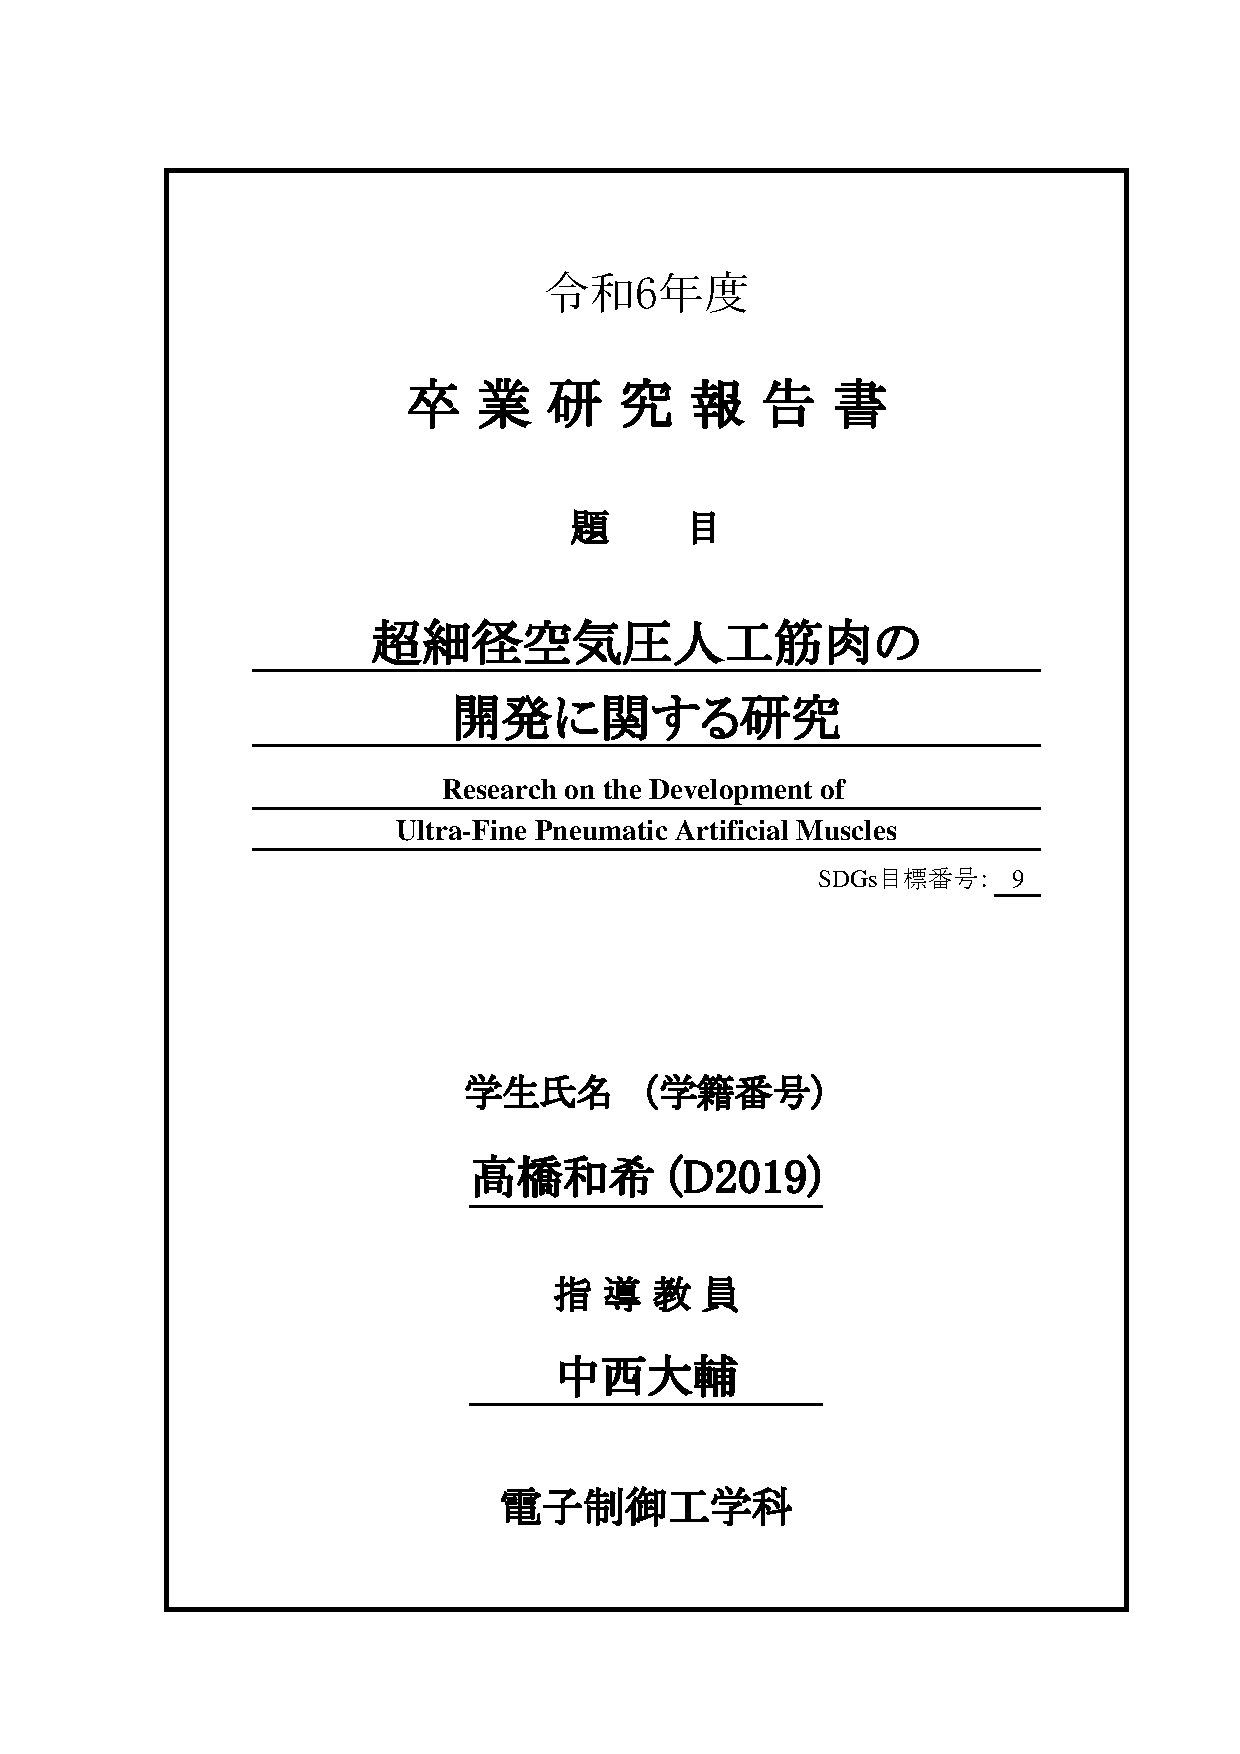
\includepdf[pages=-]{hyosi.pdf}
\thispagestyle{empty}
\newpage
\section*{概要}
        % 概要
\thispagestyle{empty}
\newpage
\section*{Abstaract}
The McKibben pneumatic actuator (MPA) is an actuator that contracts when compressed air is applied to it, generating tension in its own axial direction.
Recently, thin MPAs with a diameter of a few millimeters have been attracting attention, and their application to musculoskeletal and bio-mimetic robots has been popular because they can reproduce not only small muscles but also complex muscles by integration.
The application of MPAs to musculoskeletal and biomimetic robots is flourishing. The smallest diameter MPAs currently available on the market are those with a diameter of about 3 mm.
On the other hand, the development of even smaller diameter artificial muscles is required for further integration and application to very small robots such as small animals and insects. In this study, we focus on axial fiber-reinforced artificial muscles, which have a relatively simple structure, and aim to develop even thinner ultra-thin pneumatic artificial muscles.
This paper describes the development of a liquid lathe. In this paper, we develop a method to fabricate axial fiber-reinforced artificial muscles with inner diameters of 5 mm and 3 mm, based on our expertise in balloon fabrication using liquid latex.
The shrinkage rate and exerted tension were confirmed through experiments.

\thispagestyle{empty}
\newpage
\tableofcontents
\thispagestyle{empty}

%章ごとに呼び出し

\newpage
\setcounter{page}{1}
\section{緒言}
    % 緒言
\newpage
\section{空気圧人工筋肉}
\subsection{McKibben型空気圧人工筋肉アクチュエータ(MPA)}
MPAはシリコンゴムチューブをナイロンメッシュで覆うことで構成されており(図\ref{fig:MPA}\subref{fig:Structure}),両端に栓をするシンプルな構造である.
これに圧縮した空気を印加することでシリコンゴムチューブが膨張しメッシュによる自身の軸方向への張力が発生するアクチュエータである\cite{Yu22}(図\ref{fig:MPA}\subref{fig:move}).
高出力かつ素材自体も軽量で,物理的柔軟性による高い弾性力を持つという利点があり,筋肉の代用として生物を模したロボットやリハビリなどに用いられる.
図1に示すような直径が数10 mmのものが一般的であるが,近年では直径数 mm程度の細径タイプのMPAも普及している\cite{7989580}.細径化することで集積することが可能となり複雑な筋肉などにも
応用がされている.しかしさらなる高集積化,小動物や昆虫型などの小型なロボットへの応用を考える上ではより細径な人工筋肉の開発が求められている.しかし,現在細径MPAは最も細いもので3 mm(韓国サムスン電子グループ)
であり,また自作する場合でもナイロンメッシュは3mm程度のものが最細である.またメッシュの製作には製紐機(ブレーダー)と呼ばれる特殊な機械が必要であり,研究室で内製することは困難である.
すなわち,McKibben方式でこれ以上細径な空圧筋を作ることは困難である
%%%%%%%%%%%%%%%%%%%%%%%%%%%%%%%%%%%%%%%%%%%%%%%%%%%%%%%%%
\begin{figure}[ht]
    %
    \begin{minipage}{0.49\columnwidth}
      \vspace{4mm}
      \centering
      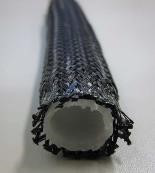
\includegraphics[scale=1]{pic/MPA_kousei.png}
      \vspace{3mm}
      \subcaption{MPA断面図}
      \label{fig:Structure}
    \end{minipage}
    %
    \begin{minipage}{0.49\columnwidth}
      \vspace{25mm}
      \centering
      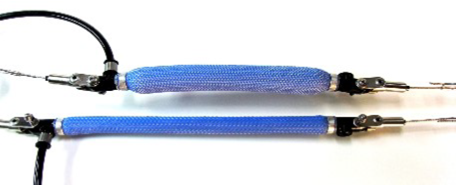
\includegraphics[scale=0.8]{pic/MPA_dousa.png}
      \subcaption{MPA外観および動作の様子}
      \label{fig:move}
    \end{minipage}
    %
    \caption{McKibben型空気圧人工筋(MPA)の構成および外観\cite{中西大輔2020}}
    \label{fig:MPA}
  \end{figure}.
\newpage
\subsection{軸方向繊維強化型人工筋肉}
そこで本研究ではMcKibbenタイプではなく,軸方向遷移強
化型の空圧筋\cite{}に着目する.軸方向繊維強化型人工筋肉の動作原理を図\ref{fig:siku}に示す.
この人工筋肉は,ゴムチューブ内に拘束繊維を内包する構造で,拘束繊維とゴムチューブとの摩耗を抑え長寿命を実現する.
空気圧が供給されると,内圧が半径方向にのみ伝達され,軸方向への効率的な収縮を引き起こす.
さらに,チューブに外挿されたリングの数を調整することで,ゴムチューブの膨張を抑制しつつ必要な収縮力を発揮できる\cite{3}
McKibbenタイプに比べ比較的構造が簡単であり市販されているナイロンメッシュの細さに細径化が左右されないためこの方式での研究を行った.
\begin{figure}[h]
  \centering  % 図全体を中央に配置
  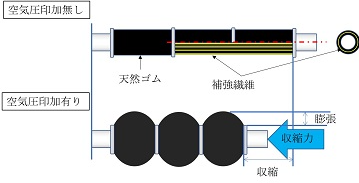
\includegraphics[scale=1]{pic/A.PNG}
  \caption{軸方向繊維強化型人工筋肉の仕組み\cite{4}}
  \label{fig:siku}
\end{figure}


            % 本文
\newpage
\section{細径MPAの開発}
\subsection{風船作製}
中西研究室では液体ゴム(前加硫ラッテクス)を用いて細径MPAを作製したことがないので,研究の第1歩として風船作製を行った.
\subsubsection{作製手順}
図3に作製に必要な物品,図4に作製手順,図5に作製した風船を示す.必要な物品は以下の通りである.
\begin{itemize}
    \item 鉄棒(内径5 mm,3 mm)
    \item REGITEX 液体ゴム(前加硫ラッテクス) メーカー:有限会社 ハイラテック
    \item PC-518用 凝固液
    \item ドライヤー Panasonic EH-Ne13
  \end{itemize}
  以下,作製手順である.
\begin{enumerate}
    \item まず初めに鉄棒を凝固液に約5秒浸して取り出す
    \item 取り出した鉄棒を凝固液の水滴がなくなるまでドライヤーで乾かす(水滴が残っているとゴムがダマになってしまいゴム厚に偏りが生じ,破裂が起きやすくなるのでよく乾かす)
    \item 鉄棒を液体ゴムに約10秒浸して取り出す(容器に鉄棒が触れるとゴムの外膜が剥がれるので注意する)
    \item 凝固液に約5秒浸して取り出す
    \item 取り出した鉄棒をゴム膜の外側のいろが白色から肌色になるまでドライヤーで乾かす
    \item 3時間程部屋で乾かしたら鉄棒からゴム膜をとる(部屋で放置しすぎるとゴムが硬くなりすぎて鉄棒から取り外すときに割れたり,穴が空きやすくなるので注意する)
\end{enumerate}
以上が本研究で用いる風船の作製手順である.
\begin{figure}[!h]
  \centering  % 図全体を中央に配置
  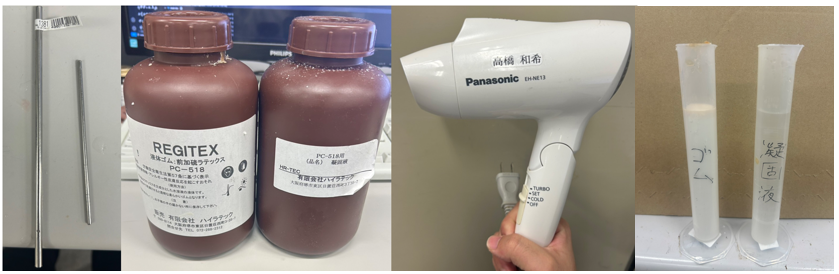
\includegraphics[scale=0.3]{pic/kigu.PNG}
  \caption{使用器具}
\end{figure}
\begin{figure}[!t]
  \centering  % 図全体を中央に配置
  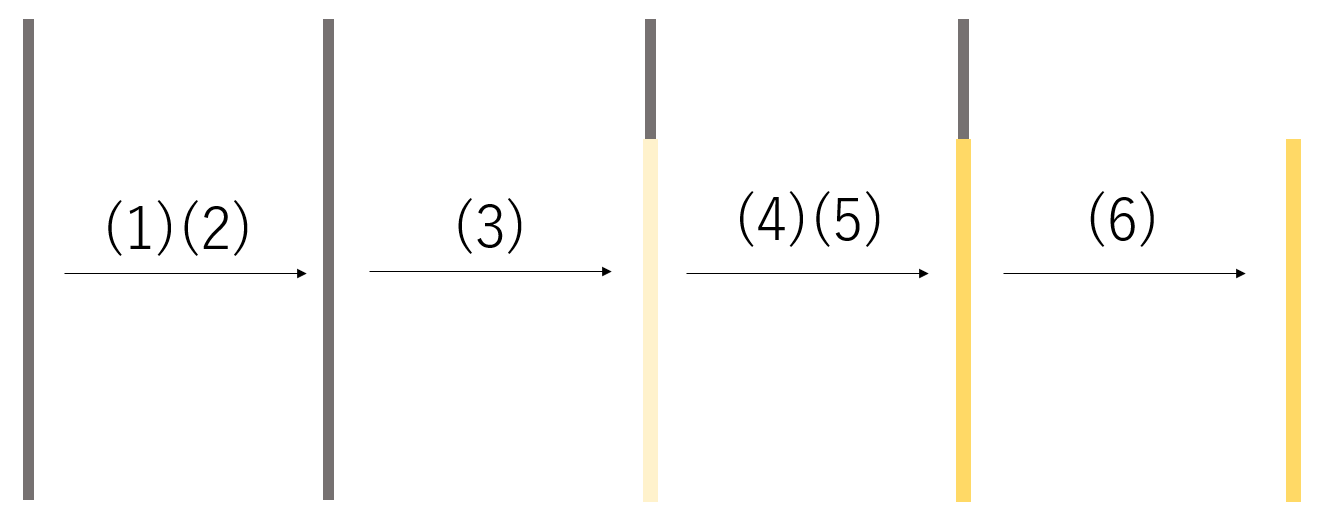
\includegraphics[scale=0.35]{pic/tezyun.PNG}
  \caption{風船の作製手順}
\end{figure}
\begin{figure}[!t]
  \centering  % 図全体を中央に配置
  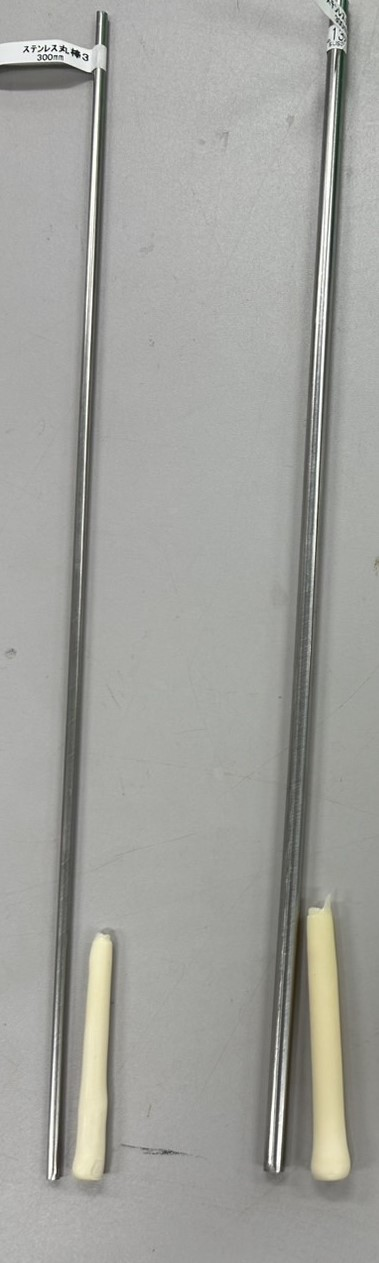
\includegraphics[scale=0.28]{pic/balloon.jpg}
  \caption{作製した風船}
\end{figure}

\newpage
\subsubsection{問題点の改善}
上記の作製方法で風船を作製するとゴム膜が硬すぎる,ゴム膜の上下で厚さにムラができる問題が生じた.この問題を解決するために以下の方法を行った.
まずゴム膜が硬すぎて膨張させることにかかる印加圧力が多く破裂が起きやすい問題に対して,ゴムと水の比率を変化させることで解決を行った.
初めはREGITEX 液体ゴム(前加硫ラッテクス)の原液のみで作製を行っていた.原液で作製を行うとゴム膜が硬すぎて図5のように破裂してしまった。
そこで実際に売られている風船と同じ比率のゴム60:水40での作製,ゴム膜が形成されるギリギリの比率を調べるためにゴム40:水60での作製を行った。
ゴム60:水40の割合で作製したゴム風船は図6のように破裂をすることなく膨張することが確認できた.一方でゴム40:水60の割合で作製したゴム風船はギリギリゴム膜を形成することができるが空圧を印加するとすぐに膨張が始まり,図7のように
破裂が生じてしまった.次にゴムの上下で厚さに差が出ている問題に対して作製方法の変更で解決を行った.図4を見れば分かるように鉄棒を液体ゴムに浸す時に1回で行っており,上下で液体ゴムに浸っている時間に差が生じてしまっていた.
そこで上と下2回に分けることで解決をした.
作製手順を以下と図8に示す.
\begin{enumerate}
  \item まず初めに鉄棒を凝固液に約5秒浸して取り出す
  \item 取り出した鉄棒を凝固液の水滴がなくなるまでドライヤーで乾かす(水滴が残っているとゴムがダマになってしまいゴム厚に偏りが生じ,破裂が起きやすくなるのでよく乾かす)
  \item 鉄棒を液体ゴムに約5秒浸して取り出す(容器に鉄棒が触れるとゴムの外膜が剥がれるので注意する)
  \item ドライヤーで凝固液の水滴がなくなるまで乾かす
  \item 鉄棒を液体ゴムに約5秒浸して取り出す
  \item 凝固液に約5秒浸して取り出す
  \item 取り出した鉄棒をゴム膜の外側のいろが白色から肌色になるまでドライヤーで乾かす
  \item 3時間程部屋で乾かしたら鉄棒からゴム膜をとる(部屋で放置しすぎるとゴムが硬くなりすぎて鉄棒から取り外すときに割れたり,穴が空きやすくなるので注意する)
\end{enumerate}

\begin{figure}[t]
  \centering
  % 上の4つの画像
  \begin{minipage}{0.49\hsize}
      \centering
      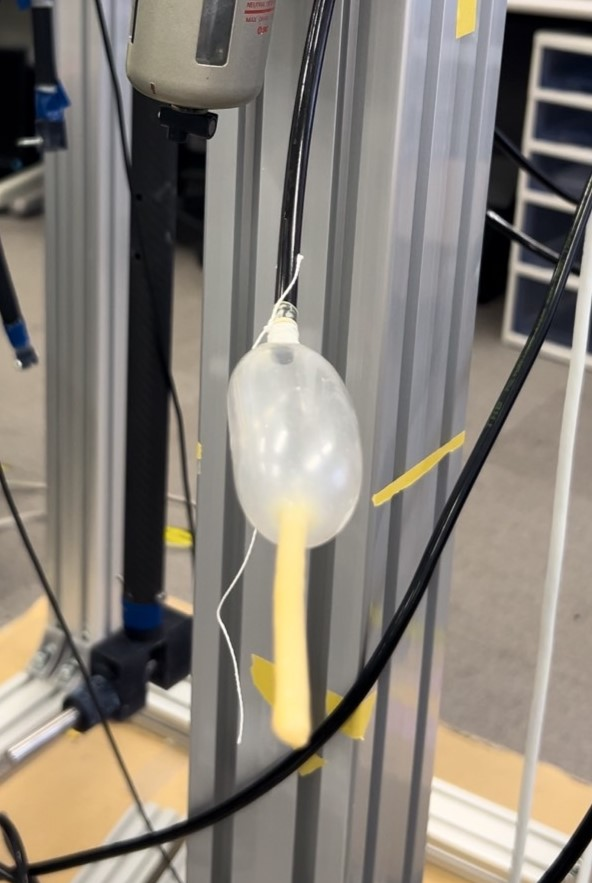
\includegraphics[scale=0.3]{pic/zu6.jpg}
      \caption{ゴム60:水40}
  \end{minipage} \hfill
  \begin{minipage}{0.49\hsize}
      \centering
      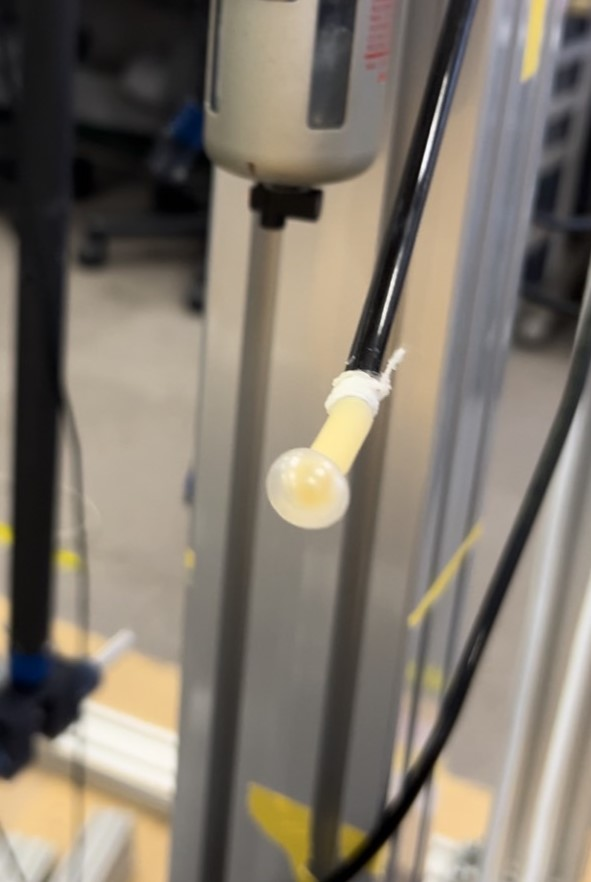
\includegraphics[scale=0.3]{pic/zu5.jpg}
      \caption{ゴム40:水60}
  \end{minipage} 
\end{figure}


\newpage
\subsection{内径5 mmの人工筋肉の作製}
超細径人工筋肉開発の開発に先立ち,まずは内径5 mmの細径空圧筋の作製を行った.作製するにあたって糸を止めるための器具を開発した.
開発した器具の写真を図9,10使用方法について図10に示す.開発した器具は図9のように鉄棒を刺す穴の周りに8つの穴が空いている.中央の穴は鉄棒より少し広い5.3 mm,糸を通す穴は1 mmで設計している.
使用方法としては図10のように鉄棒に器具をはめナイロン糸を通す仕組みになっている.
\begin{figure}[!b]
  \centering  % 図全体を中央に配置
  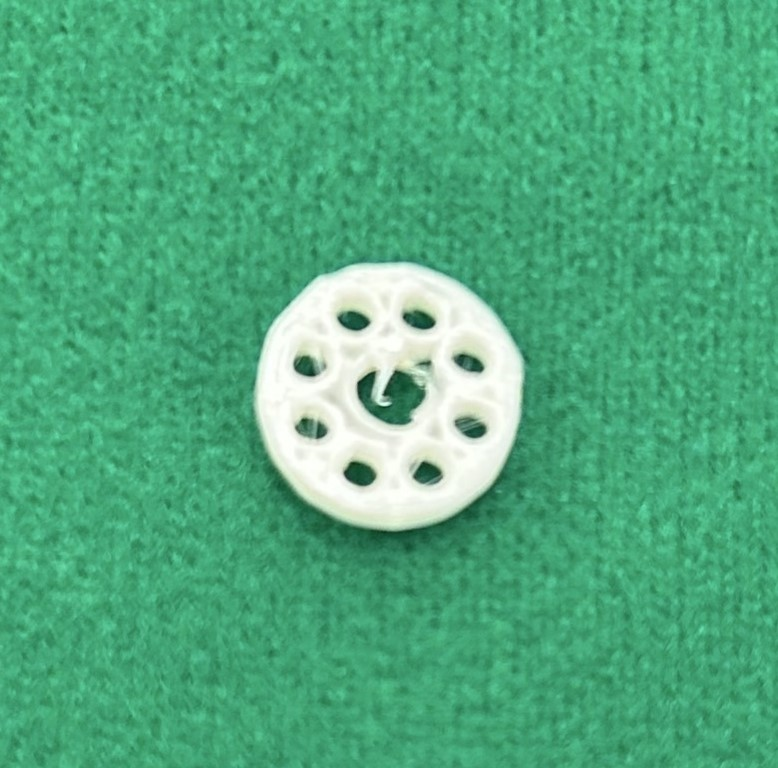
\includegraphics[scale=0.3]{pic/kigu2.jpg}
  \caption{開発した器具}
\end{figure}
\begin{figure}[!b]
  \centering  % 図全体を中央に配置
  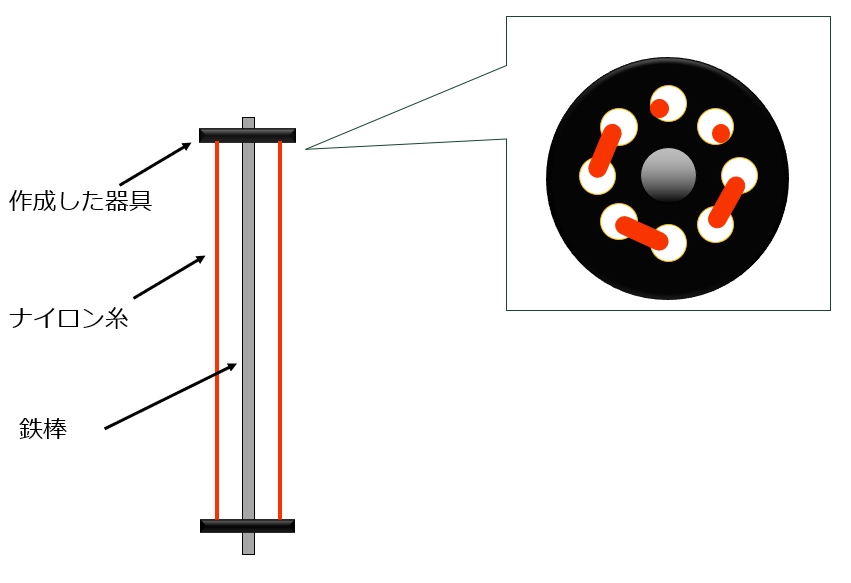
\includegraphics[scale=0.3]{pic/tukau2.PNG}
  \caption{使用方法}
\end{figure}

\begin{figure}[!b]
  \centering  % 図全体を中央に配置
  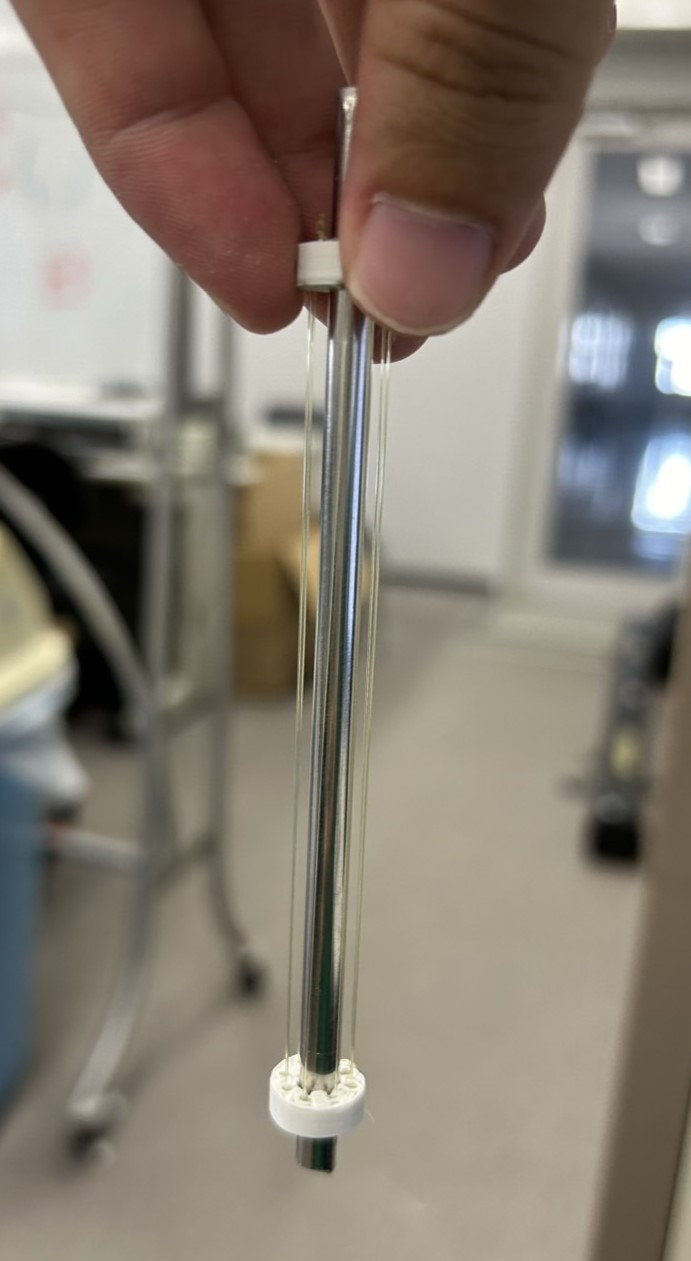
\includegraphics[scale=0.3]{pic/tukau.jpg}
  \caption{使用方法}
\end{figure}
図11に作製に必要な物品,図12,13に作製手順を示す.必要な物品は以下の通りである.
\begin{itemize}
  \item 鉄棒(内径5 mm)
  \item REGITEX 液体ゴム(前加硫ラッテクス) メーカー:有限会社 ハイラテック
  \item PC-518用 凝固液
  \item ドライヤー Panasonic EH-Ne13
  \item 道糸ナイロン 3号 200 m
  \item PPX(瞬間接着剤) メーカー:セメダイン品番:CA-522
  \item PEライン 0.4 mm
\end{itemize}

\begin{enumerate}
  \item まず初めに上記に述べた器具を鉄棒に取り付ける(固定できない場合はPPXを少し塗り,固定する)
  \item ナイロン糸を器具に通す
  \item 凝固液に約5秒浸して取り出す
  \item 凝固液の水滴がなくなるまでドライヤーで乾かす
  \item 液体ゴムに約5秒浸して取り出す
  \item ドライヤーで凝固液の水滴がなくなるまで乾かす
  \item 凝固液に約5秒浸して取り出す
  \item 取り出した鉄棒をゴム膜の外側のいろが白色から肌色になるまでドライヤーで乾かす
  \item 3時間程部屋で乾かしたら鉄棒からゴム膜をとる
\end{enumerate}
以上が本研究で作製した内径5 mmの作製手順である.作製した内径5 mmの人工筋肉を図14に示す.

\subsection{内径3 mmの人工筋肉の作製}
中間発表までの研究によって,内径5 mmの人工筋肉の作製に成功した(図14).そこでさらに細い内径3 mmの人工筋肉の開発に取り組んだ.
開発においては,中間発表までの研究に確立したベースに試行錯誤を行い,最終的に作製手順5にて作製に成功した.以下に各手法の概略と,その過程で生じた問題点について述べる.
\subsubsection{作製方法1}
作製方法1では中間発表の時と同様,鉄棒の周りに糸を張り液体ゴムに漬けることで作製を行った.
作製手順を図15,作製した人工筋肉を図16に示す.
内径が小さくなったことで図16から見て取れるように経糸同士の間隔が狭くなり,互いにくっついてしまう現象が生じた.
これによりゴム膜の幅に偏りが生じ,図17のように空圧印加時に破裂しやすくなってしまった.
\subsubsection{作製方法2}
作製方法3では糸同士の間隔が一定になるように図18のように鉄棒と縦糸の間隔を近づけて作製を行った.作製手順を以下と図19に示す.
\begin{enumerate}
  \item まず初めに器具を取り付ける
  \item ナイロン糸を器具に通す
  \item PEラインを使いナイロン糸を鉄棒に押し付ける
  \item 凝固液に約5秒浸して取り出す
  \item 凝固液の水滴がなくなるまでドライヤーで乾かす
  \item 液体ゴムに約5秒浸して取り出す
  \item ドライヤーで凝固液の水滴がなくなるまで乾かす
  \item 凝固液に約5秒浸して取り出す
  \item 取り出した鉄棒をゴム膜の外側のいろが白色から肌色になるまでドライヤーで乾かす
  \item 3時間程部屋で乾かしたら鉄棒からゴム膜をとる
\end{enumerate}
縦糸がくっつく現象は解決したものの,ゴム部内面に隙間がなくなった結果,図20のように内面側から縦糸が抜けてしまう問題が新たに発生し,軸方向への膨張を抑制することができなかった.
\subsubsection{作製方法3}
作製方法3では糸が簡単に取れなくなるように鉄棒にゴム膜を作り,その上に糸を押し付けて固定し作製を行った.
作製手順を以下と図21に示す.
\begin{enumerate}
  \item 凝固液に約5秒浸して取り出す
  \item 凝固液の水滴がなくなるまでドライヤーで乾かす
  \item 液体ゴムに約2秒浸して取り出す
  \item 凝固液に約5秒浸して取り出す
  \item 凝固液の水滴がなくなるまでドライヤーで乾かす
  \item 液体ゴムに約2秒浸して取り出す
  \item 凝固液に約5秒浸して取り出す
  \item 凝固液の水滴がなくなるまでドライヤーで乾かす
  \item 器具を取り付ける
  \item ナイロン糸を器具に通す
  \item PEラインを使いナイロン糸をゴム膜に押し付ける
  \item 凝固液に約5秒浸して取り出す
  \item 凝固液の水滴がなくなるまでドライヤーで乾かす
  \item 液体ゴムに約5秒浸して取り出す
  \item ドライヤーで凝固液の水滴がなくなるまで乾かす
  \item 凝固液に約5秒浸して取り出す
  \item 取り出した鉄棒をゴム膜の外側のいろが白色から肌色になるまでドライヤーで乾かす
  \item 3時間程部屋で乾かしたら鉄棒からゴム膜をとる
\end{enumerate}
内面側から糸が抜ける問題は改善したものも糸がある場所で図22のようにゴム膜が2つの層に分かれてしまい,強度が低下し破裂が生じ
てしまった.
\subsubsection{作製方法4}
糸を入れてないときは層ができてなかったので,糸にゴムをコーティングすれば糸がある場所に層ができないと考えた.
図23に作製に必要な物品,図24に糸にゴムをコーティングする方法を示す.必要な物品は以下の通りである.
\begin{itemize}
  \item REGITEX 液体ゴム(前加硫ラッテクス) メーカー:有限会社 ハイラテック
  \item PC-518用 凝固液
  \item 作製した器具
  \item アーマードF+pro 0.06号
  \item 綿 手縫い糸
  \item オーブントースター CF-AC121
\end{itemize}
以下,作成手順である
\begin{enumerate}
  \item 糸を図25のように巻きつける
  \item 凝固液に約5秒浸して取り出す
  \item 凝固液の水滴がなくなるまでドライヤーで乾かす
  \item 液体ゴムに約10秒浸して取り出す
  \item 凝固液に約5秒浸して取り出す
  \item オーブントースターで80度で10分乾かす
\end{enumerate}
この方法で作製した糸を用いて作製方法3と同様な方法で作製を行った.また今回からオーブンを使用して乾燥を行った.
図26からみて分かるように糸をゴムでコーティングしても層ができる現象は改善されなかった.
\subsubsection{作製方法5}
作製方法5ではゴムが2層になる問題を回避するために,作製方法1と同様1度にゴム膜を形成する方法に戻した.
また糸がくっつく問題を回避するために,縦糸にテンションをかけるネジを用いた器具を開発した.
開発した器具の使用方法を図27,28に示す.

作製方法を以下に示す.
\begin{enumerate}
  \item 器具を鉄棒に取り付ける
  \item 器具に糸を通しネジを回すことで糸にテンションをかける
  \item 凝固液に約5秒浸して取り出す
  \item 凝固液の水滴がなくなるまでドライヤーで乾かす
  \item 液体ゴムに約10秒浸して取り出す
  \item 凝固液に約5秒浸して取り出す
  \item 取り出した鉄棒をゴム膜の外側のいろが白色から肌色になるまでドライヤーで乾かす
 \item 時間程部屋で乾かしたら鉄棒からゴム膜をとる
\end{enumerate}
作製方法4ではオーブンで乾かすことによりゴム膜を硬くしていたが,硬くなることによって膨張が起きにくくなっていたので部屋でゆっくりと乾燥させる方式に戻した.
作製した人工筋肉は図29のように糸のくっつきおよび2層化の問題は生じなかった.また印加圧力によって空圧筋として動作することが確認した.

 



\newpage
\section{評価実験}
\subsection{収縮率}
\subsubsection{内径3 mmの測定}
図\ref{fig:zA}に今回作製した内径3 mmの人工筋肉を示す.
測定方法は内径5 mmの測定と同様な方法で行った.
空圧を印加すると0.06Mpaが膨張の最大となった.
空圧印加前の長さは54 mm,空圧印加後の長さは49 mmで収縮率を求める式に代入すると
$$\frac{(49 \rm{mm})-(54 \rm{mm})}{49 \rm{mm}}\times 100\\$$
となり収縮率が9.3 \%となることが確認できた.
\begin{figure}[h]
    %
    \begin{minipage}{0.49\columnwidth}
      \vspace{4mm}
      \centering
      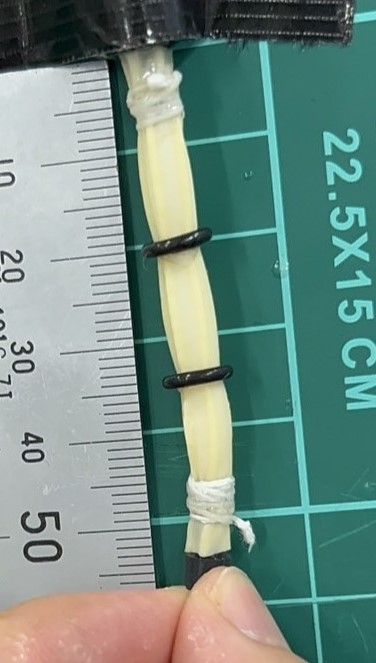
\includegraphics[scale=0.3]{pic/M.jpg}
    
      \subcaption{空圧印加前}

    \end{minipage}
    %
    \begin{minipage}{0.49\columnwidth}
      \vspace{4mm}
      \centering
      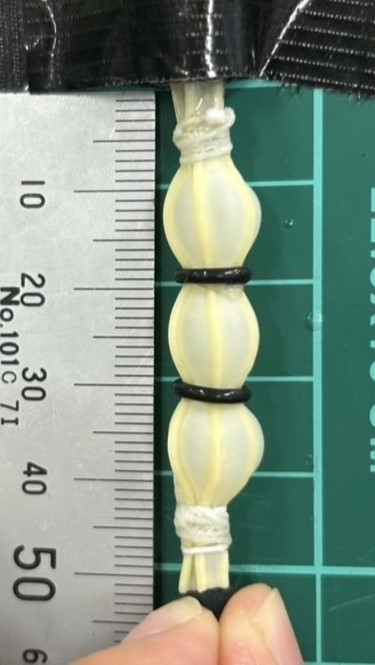
\includegraphics[scale=0.3]{pic/L.jpg}
      \subcaption{空圧印加後}
      
    \end{minipage}
    %
    \caption{内径3 mmの人工筋肉}
    \label{fig:zA}
  \end{figure}.
\subsection{発揮張力}
図\ref{fig:souti},\ref{fig:souti2}のような装置を使い発揮張力の測定を行った.またケブラーラインを通すために人工筋肉の先に図\ref{fig:new}を取り付けた.穴の直径は3 mmほど空いている.
測定に必要な物品は以下の通りである.
\begin{itemize}
  \item 作製した人工筋肉
  \item 万力
  \item S字フック
  \item 電子天秤 I 2000
\end{itemize}
測定手順を以下に示す.
\begin{enumerate}
  \item 作製した人工筋肉にケブラーラインを通す
  \item S字フックを取り付け電子天秤につなぐ
  \item 糸にテンションがかかる位置で万力に人工筋肉を固定する
  \item 電子天秤に電源をつけ,0点合わせをする
  \item 膨張の最大まで印加し,その時点での値を読み取る
\end{enumerate}
上記の手順で測定を行うと0.07Mpa印加した際に膨張が最大となり,その時点での電子天秤の値は138.4 gとなった図\ref{fig:138}.
このことから今回作製した人工筋肉が138.4 gまで持ち上げ可能な特性を有していることが確認できた.
\begin{figure}[h]
  %
  \begin{minipage}[b]{0.49\columnwidth}
    \vspace{4mm}
    \centering
    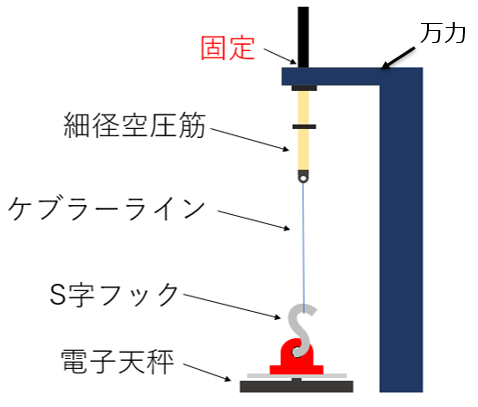
\includegraphics[scale=0.5]{pic/souti.PNG}
  
    \caption{測定装置のイメージ}
    \label{fig:souti}
  \end{minipage}
  %
  \begin{minipage}[b]{0.49\columnwidth}
    \vspace{8mm}
    \centering
    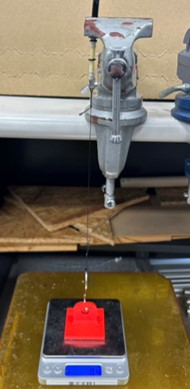
\includegraphics[scale=0.8]{pic/new.jpg}
    \caption{測定装置}
    \label{fig:souti2}
  \end{minipage}
  %
\end{figure}.
\begin{figure}[h]
  %
  \begin{minipage}{0.49\columnwidth}
    \vspace{4mm}
    \centering
    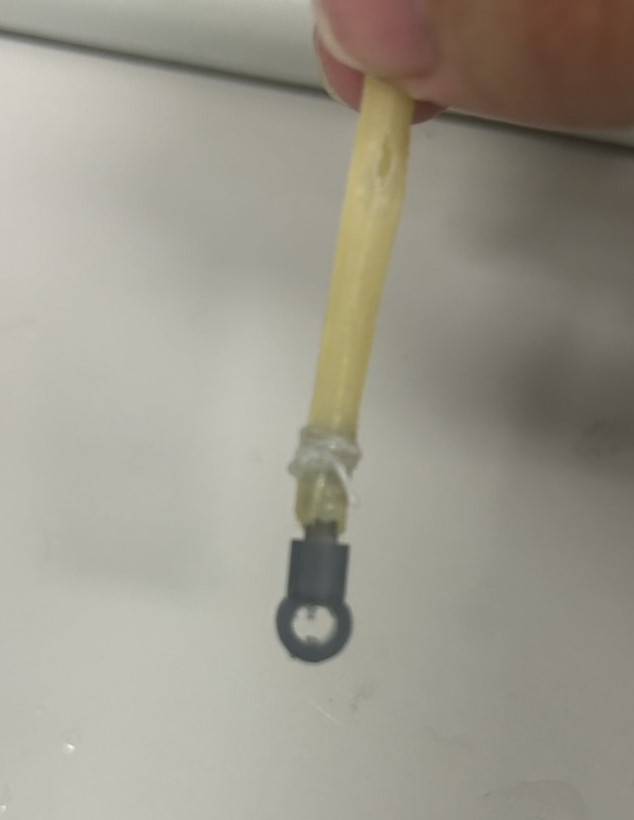
\includegraphics[scale=0.2]{pic/gg.jpg}
    \caption{開発した器具}
    \label{fig:new}
  \end{minipage}
  %
  \begin{minipage}{0.49\columnwidth}
    \vspace{4mm}
    \centering
    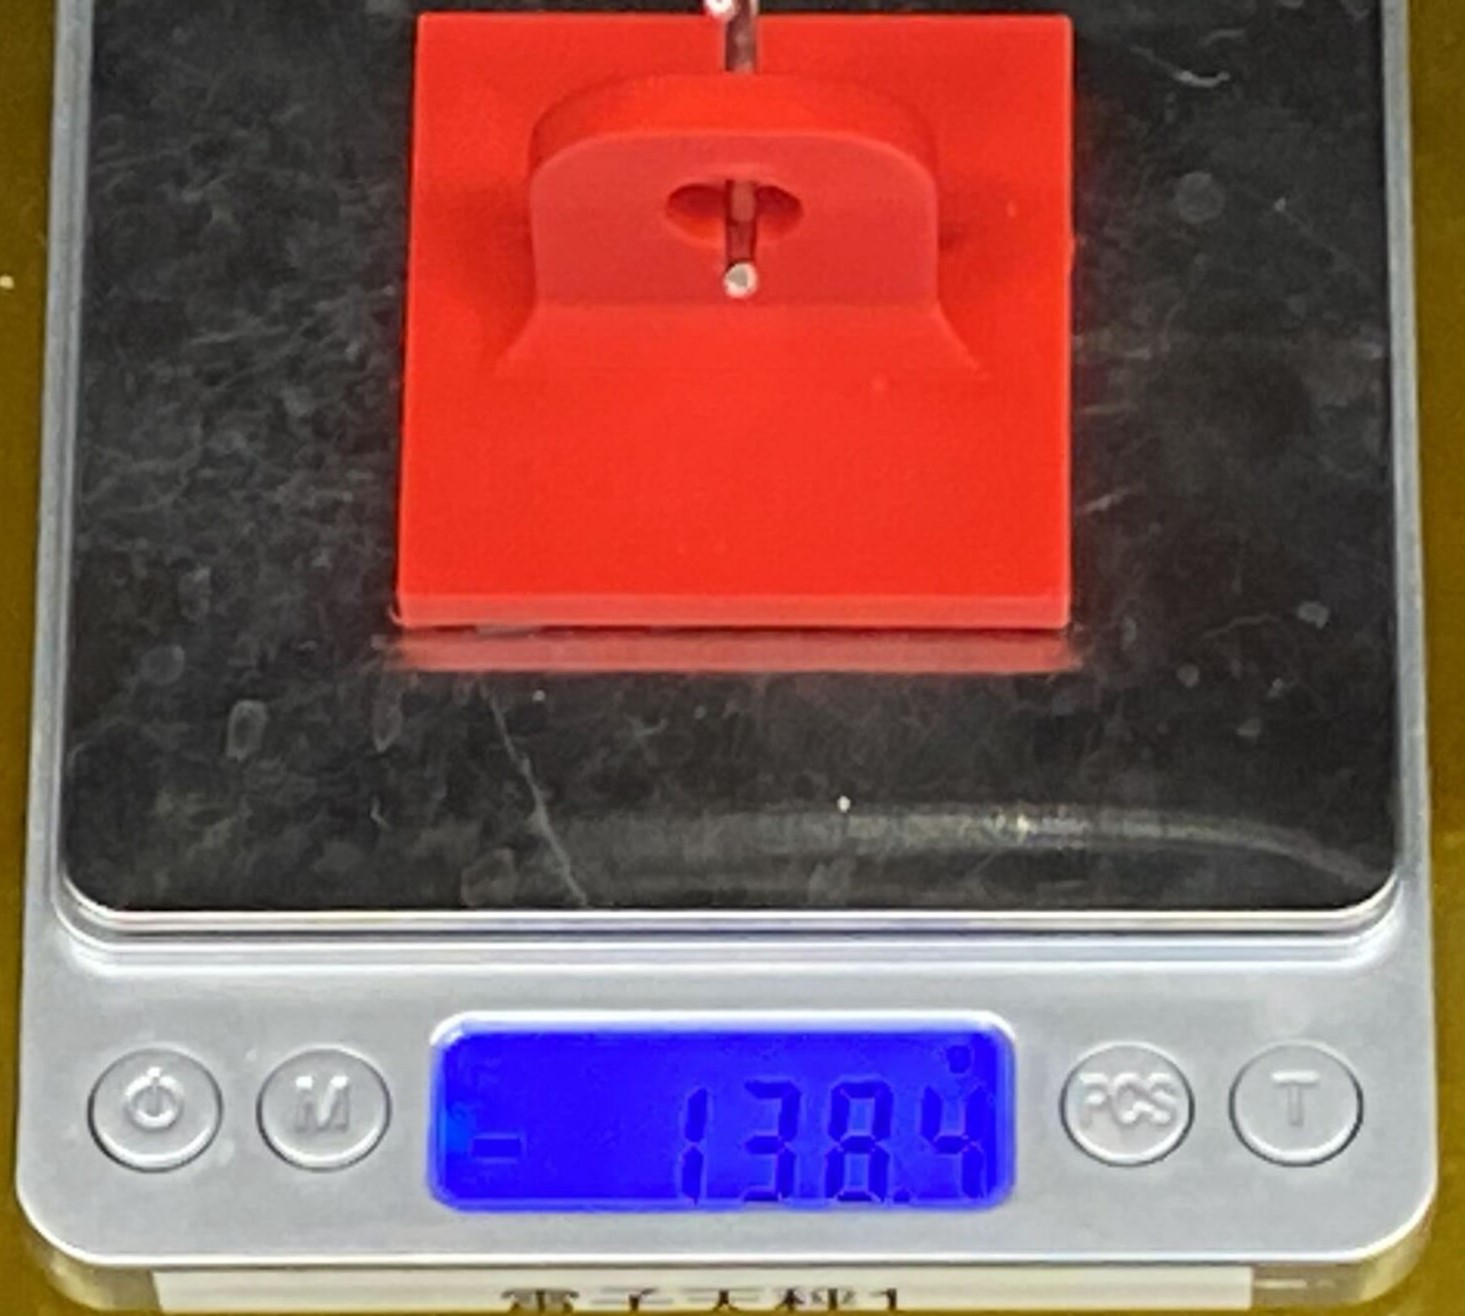
\includegraphics[scale=0.1]{pic/qqqq.jpg}
    \caption{電子天秤の値}
    \label{fig:138}
  \end{minipage}
  %
\end{figure}.

\newpage
\section{考察}
一般的な軸方向繊維強化型空気圧人工筋肉において
は,ゴムの膜厚は均一であり,その内部に縦糸が配置さ
れていることが一般的である.本研究でも,なるべくゴ
ム厚が均一になるよう,また糸がゴム膜の中に収まるよ
う作製方法を模索していった(図\ref{fig:mmm}\subref{fig:44}).
一般的な軸方向繊維強化型空気圧人工筋肉において
は,ゴムの膜厚は均一であり,その内部に縦糸が配置さ
れていることが一般的である.本研究でも,なるべくゴ
ム厚が均一になるよう,また糸がゴム膜の中に収まるよ
う作製方法を模索引き起こす結果となった.一方で,空圧筋として動作を
確認した作成方法5で作製した空圧筋(図\ref{fig:mmm}\subref{fig:44})においては,
糸はゴム膜の中央には配置されておらず,糸と糸
の間に薄いゴム膜を張るような構成となった.このこと
により,膨張がスムーズに行われ,空圧筋が高い柔軟性
を持ちながらも,必要な強度を確保することができた.
よって,今後より細径な空圧筋を開発する上ではゴム膜
の厚さと糸配置のバランスを取ることが重要であり,(図\ref{fig:mmm}\subref{fig:55})
のようにひだ状に作っていくことが有効であると
考えられる.
\begin{figure}[h]
  \centering
  % 上の4つの画像
  \begin{minipage}{0.49\textwidth}
      \centering
      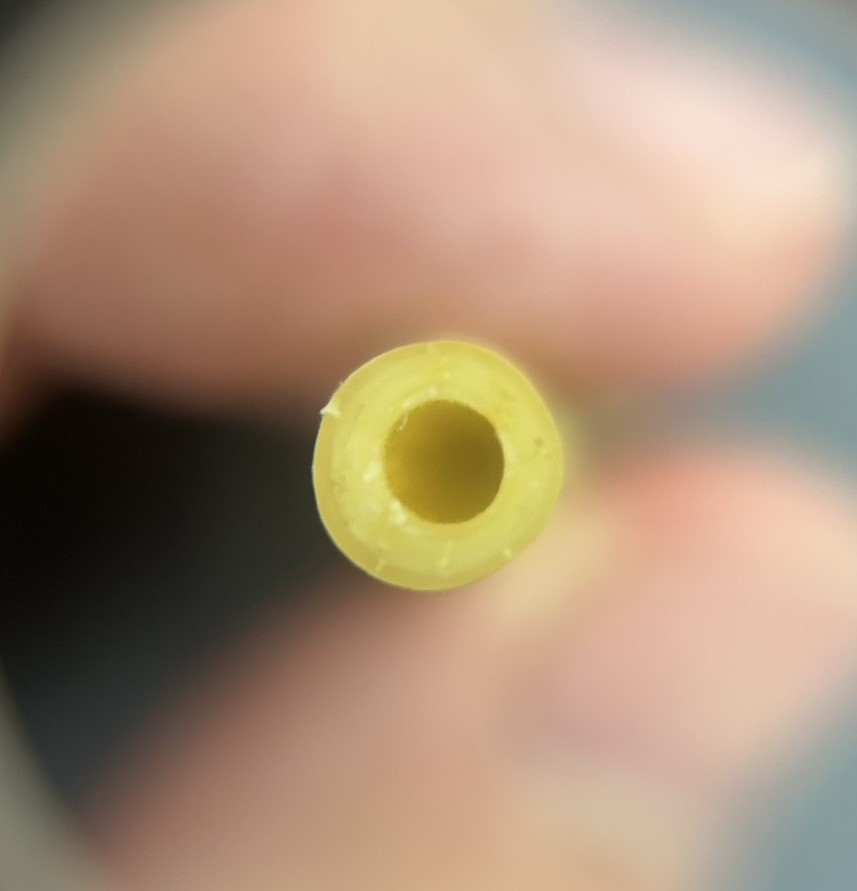
\includegraphics[scale=0.3]{pic/O.jpg}
      \subcaption{作成方法4}
      \label{fig:44}
  \end{minipage} \hfill
  \begin{minipage}{0.49\textwidth}
      \centering
      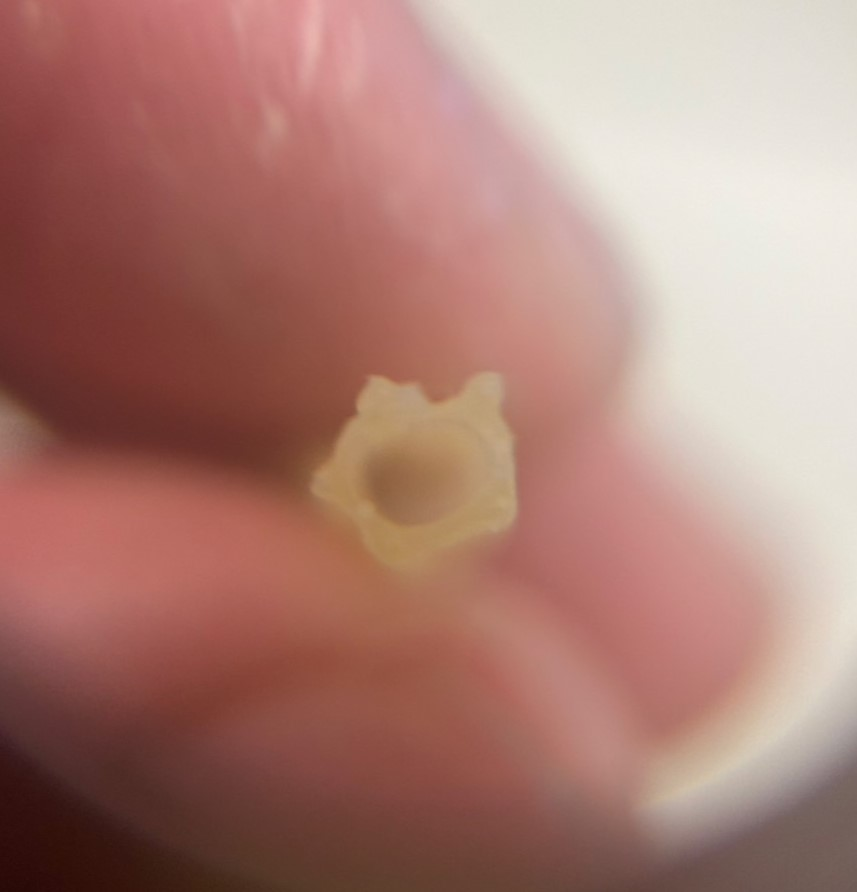
\includegraphics[scale=0.3]{pic/P.jpg}
      \subcaption{作成方法5}
      \label{fig:55}
  \end{minipage} 
  \caption{作成した細径空圧筋の断面}
  \label{fig:mmm}
\end{figure}


% 必要に応じて章を増やす,またファイル名もsec2, sec3である必要はない
% このmain.texが置いてあるディレクトリ内にある「chapters」フォルダ以下に
% 自分がわかりやすい名前のtexファイルを作成し,\include{chapters/*****}で
% 呼び出せば良い
\newpage
\section{結言}

本研究では,ゴム皮膜を用いた軸方向繊維強化型人工筋肉による,超細径空気圧人工筋肉の開発を目的として研究を行った.
まず液体ゴムを用いて細径風船の作製を行い,凝固液の適切な乾かし方,液体ゴムに浸す時間についての知見を得た.
その後最適なゴムと水の割合,ムラのできない作製方法の確立を行った.次に内径5 mmの人工筋肉の作製を行いゴム被膜に糸を内包するノウハウを得た.
そのノウハウを生かして様々な作製方法を模索し,内径3 mmの人工筋肉の作製に成功した.最後に評価実験を行い,収縮率が9.3 \%,発揮張力が138.4 gであることが確認でき,空圧筋として動作した.
\noindent

今後はより細径な軸方向繊維強化型人工筋肉を目指すとともに性能の向上に取り組む予定である.
      % 結言
\newpage
\section{謝辞} % 謝辞
% できればbibtexを使ってください

\newpage
\bibliographystyle{junsrt}
\bibliography{sanko.bib}


    % 参考文献

\end{document}
